\chapter{Effect of statistical uncertainties}
\label{cha:stat_unc}

% **************************** Define Graphics Path **************************
\ifpdf
    \graphicspath{{Chapter3/Figs/Raster/}{Chapter3/Figs/PDF/}{Chapter3/Figs/}}
\else
    \graphicspath{{Chapter3/Figs/Vector/}{Chapter3/Figs/}}
\fi

% **************************** Chapter Abstract ******************************
\leftskip=1cm
\noindent
\emph{This chapter studies the effect of commonly neglected statistical uncertainties on representative fractiles and on structural reliability. The failure probability of a generic structural member, subjected to snow load is analyzed using frequentist and Bayesian techniques to quantify parameter estimation and model selection uncertainties in ground snow load. Various variable to dead load ratios are considered to cover a wide range of real structures. The analysis reveals that statistical uncertainties may have a substantial effect on  reliability. By accounting for  parameter estimation uncertainty,  the failure probability can increase by  more than  an  order  of  magnitude. Bayesian posterior predictive distribution is recommended to incorporate parameter estimation uncertainty in reliability studies.}

\leftskip=0pt\rightskip=0pt

%****************************************************************************************
%****************************************************************************************
\section{Problem statement and the state of the art}

One of the main concerns in structural reliability is the calculation of very small probabilities, such as events expected to occur once in 10000 years. A major difficulty in this is that actions, which structures should withstand, are inferred from 50-100 years of observations. This information might be supplemented by phenomenological or theoretical models but these are seldom available or far too complex to be used in engineering design. 

Hence, probabilistic models of actions are affected by substantial uncertainty, which might dominate the reliability \citep{Coles2003catastrophes}. These uncertainties, which are related to the identification of the probabilistic model on the basis of limited data, are referred hereinafter as statistical uncertainties. Only modeling of a random variable is considered, hence the statistical model uncertainty means the uncertainty in the selection of probabilistic model (distribution function), and the statistical parameter estimation uncertainty refers to the uncertainty in the identification of unknown parameters (e.g. location, scale, shape) of a particular distribution. These two are not entirely separable but it is convenient to use both terms. Statistical uncertainties stem from the scarcity of available information and inevitably present for every probabilistic models. For simplicity they are referred to as parameter estimation and model selection uncertainties.

In reliability studies and standardization statistical uncertainties are routinely neglected \citep{Sanpaolesi1998, Coles2003fully_prob, Sisson2006}. However, this violates a basic requirement of probability calculation, namely that all information should be incorporated and all uncertainties accounted for \citep{Kiureghian1989}. The aim of this section is to explore the effect of this omission on selected fractiles and on structural reliability. Moreover, it critically compares some statistical approaches to incorporate statistical uncertainties into probabilistic models.

%Although the practical calculations are performed on snow extremes, it is expected that the findings can be beneficial for other extremes as well, e.g. there is an ongoing revision of wind loads in Eurocode (WG7) with many overlapping challenges with those of snow loads.

%Hence, the probabilistic models are subjected to substantial statistical uncertainties, i.e. uncertainty in model selection and uncertainty in parameter estimation The current civil engineering practice typically neglects these uncertainties or inadequately addresses them.

%****************************************************************************************
%****************************************************************************************
\section{Solution strategy}
The meteorological actions on structures are almost solely described by statistical distributions since the underlying natural phenomena are too complex to be represented by physical models. This approach is adopted here and the ground snow load intensity is modeled by a single random variable.
  
In line with the current engineering practice the block method \citep{Coles2001} is applied. The block length is one year, covering a whole winter season. The annual ground snow maxima are treated as a sample for each location. The potentially more effective multiple block maxima or smaller block lengths are discarded, since the accumulative nature of snow loads makes it difficult to identify peaks and to justify their independence. For the same reason the peak over threshold approach \citep{Reiss2007} was also not used. To account for dependence between maxima from the same winter season a stochastic process based approach is presented in Chapter~\ref{cha:copula}.

For other actions the dependence of maxima is typically lower, thus multiple block maxima and peak-over threshold approaches are advised to be considered. These methods often extends the sample size by orders of magnitude, thus might substantially reduce statistical uncertainties. For wind speed maxima it is demonstrated that these approaches can lead to 70\% reduction in confidence interval for 1000-year fractiles compared with the annual block maxima approach \citep{RozsasREC2016wind}.

Since the main goal of this chapter is to demonstrate the effect of neglecting statistical uncertainties we believe that it is sufficient to use the one year block approach. This creates common ground for comparison, though in future works approaches that use more information should be considered.

Observations from the Carpathian Region are used to infer the distribution parameters (Section~\ref{sec:data_under_study}). The statistical and structural reliability machinery presented in Section \ref{cha:overview} is utilized to explore the effect of statistical uncertainties on representative fractiles and on structural reliability, and to identify the appropriate distribution type for ground snow maxima.

%\mynote{praise the approach compared to studies where the representative values interpolated}
%The widespread approach is to use the measurements of meteorological stations, infer representative values, and spatially interpolate them to obtain maps. In contrast, here the gap filling is done through interpolation and using meteorological models in space and time too on the level of daily snow water equivalent observations. With the exception of analyzing the maxima these analyses are done by meteorologists and provided in a database (ref).
%Turkey - ASCE \citep{Durmaz2006}

%****************************************************************************************
%****************************************************************************************
\subsection{Data under study}
\label{sec:data_under_study}
The meteorological data are obtained from the CarpatClim database, which is the outcome of a cooperation between nine countries of the Carpathian Region \citep{Szalai2013}. The research is completed under the leadership of the Hungarian Meteorological Service that coordinated the joint effort of the meteorological institutions of Austria, Croatia, Czech Republic, Poland, Romania, Serbia, Slovakia and Ukraine.

The database provides snow water equivalents (SWE) in about 10~km  spatial and daily temporal resolution that corresponds to the period from 1961 to 2010. The daily maxima are recorded in the database. The climatological grid covers the region between latitudes 44°N and 50°N, and longitudes 17°E and 27°E (Figure~\ref{fig:carp_stations}-\ref{fig:elevation_map}). The data are gathered from 288 climate stations and 355 precipitation stations with relatively homogeneous spatial distribution. These are homogenized and spatially interpolated using meteorological and  statistical models, missing data are also filled in using these models. The post-processed data are available in the database. 


\mynote{on the slides of Mónika Lakatos 415 climate stations and 904 precipitation stations are mentioned, this is in conflict with the official website of the project;
missing data is filled by model predictions, should be added}

\begin{figure}[htbp!]
	\centering    
	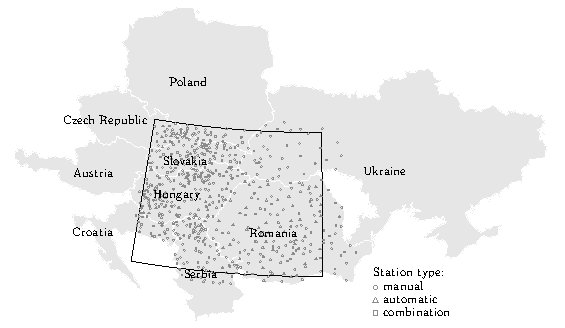
\includegraphics[width=1\textwidth]{carp_map_stations_ai.pdf}
	\caption{Illustration of the studied region (black frame) with involved countries and meteorological stations.}
	\label{fig:carp_stations}
\end{figure}

\begin{figure}[htbp!]
	\begin{subfigure}[b]{0.49\textwidth}    
		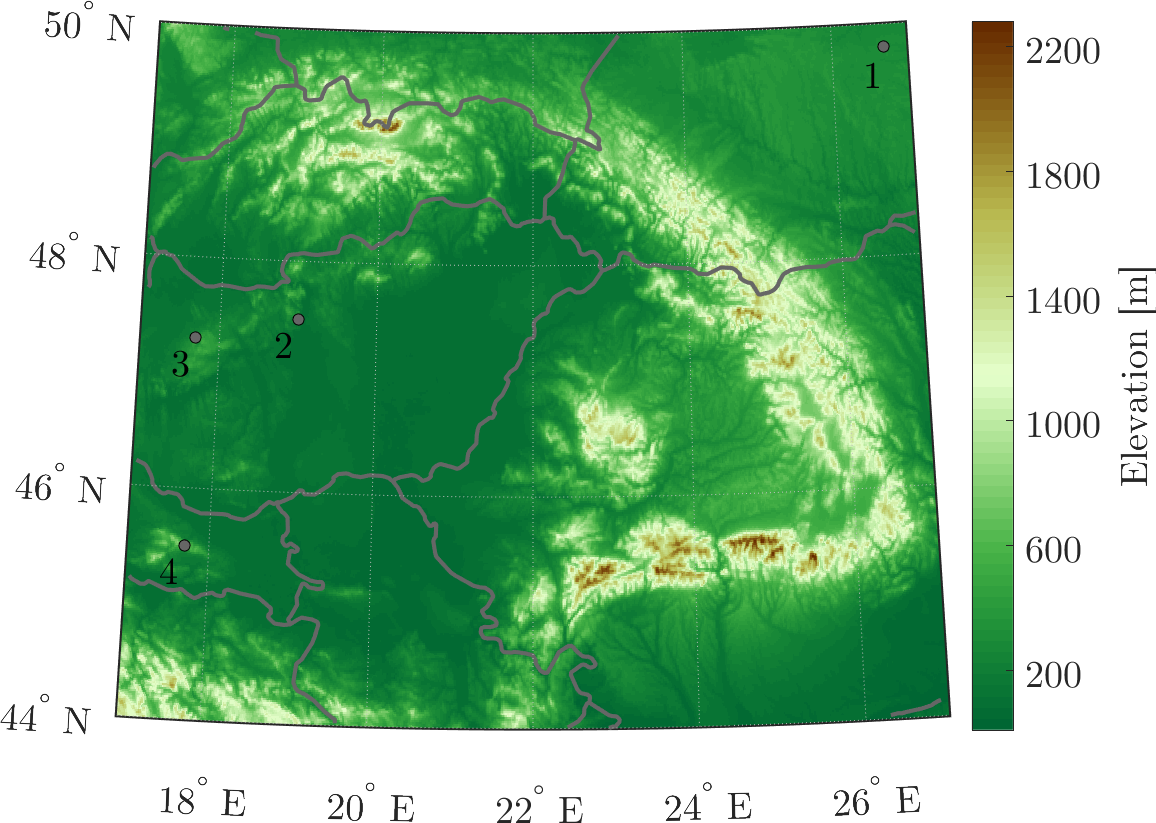
\includegraphics[width=\textwidth]{elevation_map_carpathian_region.png}
		\caption{Elevation map.}
		\label{fig:elevation_map}
	\end{subfigure}
	\hfill
	\begin{subfigure}[b]{0.49\textwidth}
		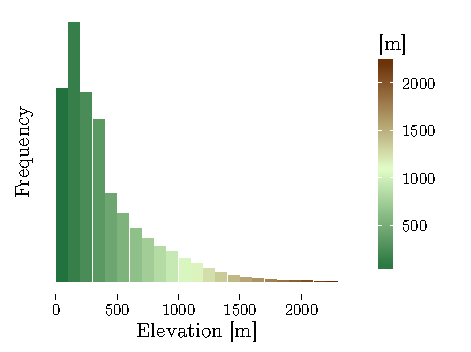
\includegraphics[width=\textwidth]{hist_elevation.pdf}
		\caption{Elevation histogram.}
		\label{fig:elevation_hist}
	\end{subfigure}
	\caption{Illustration of the studied Carpathian region with elevation data with selected locations' ID (Table~\ref{tab:loc_parmest}).}
\end{figure}

Information about the available snow water equivalent data is taken verbatim from the supplementary document of the CarpatClim project \citep{Szalai2013}:
\begin{itemize}
	\item[] ``The water equivalent of a snow cover is the vertical depth of the water that would be obtained by melting the snow cover \citep{WMO2008}.''
	\item[] ``a snow cover model employed operationally at ZAMG [Central Institution for Meteorology and Geodynamics, Austria], was applied to generate a 0.1° latitude/longitude grid of daily mean snow cover and corresponding estimated water equivalent and snow depth simulations. The applied model is based on pre-finished CARPATCLIM grids of mean air temperature [°C], precipitation sum [mm] and relative air humidity [\%]. They are processed by the snow cover model regarding three main parts \textit{accumulation of snow cover, ablation of snow cover and transformation of SWE to snow depth} [emphasis in the original].''
\end{itemize}
Further details about the applied procedures can be found in the cited document.

Uncertainty due to measurement error and due to the approximate nature of meteorological models are neglected. Unless otherwise noted this approach is taken in all chapters, Chapter~\ref{cha:error} deals with this issue in details.


\mynote{images should be improved, country names should be added + precipitation and climate stations}

%****************************************************************************************
%****************************************************************************************
%\section{Distribution of annual ground snow maxima}
%
%In respect of the distribution of ground snow maxima no international consensus has been reached so far. Some commonly used distribution types with regions:
%\begin{itemize}
% \item In Europe Gumbel distribution is typical, it is used for constructing characteristic ground snow maps for most CEN countries \citep{Sanpaolesi1998}.
% \item The Czech Republic derived its snow map using three-parameter Lognormal distribution \citep{Krivy2010}.
% \item In the United States two-parameter Lognormal distribution is adopted in \cite{ASCE2010} based on the research of \citet{Ellingwood1984}.
% \item In Colorado state Normal, Gumbel, three-parameter Lognormal, three-parameter Fréchet, three-parameter Gamma, and three-parameter Loggamma distributions are used and various statistical goodness-of-fit measures are used to select the most appropriate for each site \citep{SEAC2007}.
%\end{itemize}
%Countries even with similar climatic conditions often use different types that typically yield to similar characteristic values but their tail -- governing the failure probability -- is substantially different.
%
%%****************************************************************************************
%\subsubsection*{Generalized extreme value distribution, GEV}
%
%The mathematical support is given by the extreme value theory that states that independent, identically distributed block maxima will asymptotically converge to the generalized extreme value family, irrespectively of the parent distribution \citep{Coles2001, Reiss2007}.
%The standard parametrization of GEV distribution is used with shape ($\xi$), scale ($\sigma$) and location ($\mu$) parameters, see Appendix~\ref{ap:prob_models}, Eq.~\ref{eq:gev_cdf}. The GEV distribution family comprises three special types: Weibull ($\xi < 0$), Gumbel ($\xi = 0$) and Fréchet ($\xi > 0$), see Figure~\ref{fig:gev_skewness}. The first has an asymptotic upper bound while the latter two are unbounded.
%
%
%\subsubsection*{Lognormal distribution}
%
%It is a heavy tailed distribution with $[0,\infty]$ domain that fits better to the majority of the natural phenomena than the typical domain of GEV. Nevertheless, it is not supported by theoretical considerations and unbounded over its whole parameter domain.
%
%The three-parameter Lognormal is the generalization of two-parameter Lognormal by adding a third parameter that shifts the distribution on horizontal axis \citep{Singh1998}.


%****************************************************************************************
\section{Effect on representative fractiles}
Parameter estimation and model selection uncertainty quantifications are conducted for multiple locations of the Carpathian Region. The results of three representative locations are presented in more details: Location 1, 2 and 3 are identified as likely belonging to Weibull, Fréchet and Gumbel families, respectively (Table~\ref{tab:loc_parmest}). To examine the annual ground snow load of other locations an online, interactive snow map is developed by the candidate (Annex~\ref{sec:int_snow_map}). Among others, it can be used to explore the effect of statistical uncertainties and to obtain characteristic ground snow loads.

\begin{table}[htbp!]
\caption{Characteristics of selected locations to illustrate the effect of statistical uncertainties on representative fractiles.}
\centering
\label{tab:loc_parmest}
\small
	\begin{threeparttable}
    \begin{tabular}{l l l l l}
    \toprule
    Location ID\tnote{*}  & Description & Representative of & Elevation [m] & Coordinates  \\
    \midrule
    \rowcolor{lightgrey} 1 (300)  & Ukraine, highland & Weibull & 299 & 49.8°N 26.7°E   \\
    2 (2735)  & Hungary, lowland & Fréchet & 241 & 47.3°N 17.7°E   \\
    \rowcolor{lightgrey} 3 (4553)  & Croatia, highland & Gumbel & 753 & 45.5°N 17.7°E   \\
    4 (2546)  & Hungary, lowland & Fréchet\tnote{\textdagger} & 226 & 47.5°N 19.0°E   \\
    \bottomrule
    \end{tabular}
    \begin{tablenotes}
        \item[*] The first number is used as an identifier here, while the second -- in brackets -- is related to the database.
        \item[\textdagger] Ambiguous, close to Gumbel.
    \end{tablenotes}
    \end{threeparttable}
\end{table}


Two-parameter Lognormal (LN2), three-parameter Lognormal (LN3), Gumbel and Generalized extreme value (GEV) distributions are selected for the comparative analysis (see Annex \ref{sec:distr_fun}). The LN2 model is typically adopted in the USA \citep{ASCE2010} based on the research of \citet{Ellingwood1984}, while the Czech Republic derived its snow map using LN3 distribution \citep{Krivy2010}. The Gumbel model is wide-spread in Europe \citep{Sanpaolesi1998, JCSS_load}. The GEV distribution comprises the Gumbel as a special type and it is supported by the extreme value theory \citep{Coles2001}. The standard parametrization of GEV distribution is used with shape ($\xi$), scale ($\sigma$) and location ($\mu$) parameters, see Appendix~\ref{sec:distr_fun}, Eq.~\ref{eq:gev_cdf}. The GEV distribution family comprises three special types: Weibull ($\xi < 0$), Gumbel ($\xi = 0$) and Fréchet ($\xi > 0$), see Figure~\ref{fig:gev_skewness}. The first has an asymptotic upper bound while the latter two are unbounded.

\begin{figure}[htbp!]
	\centering    
	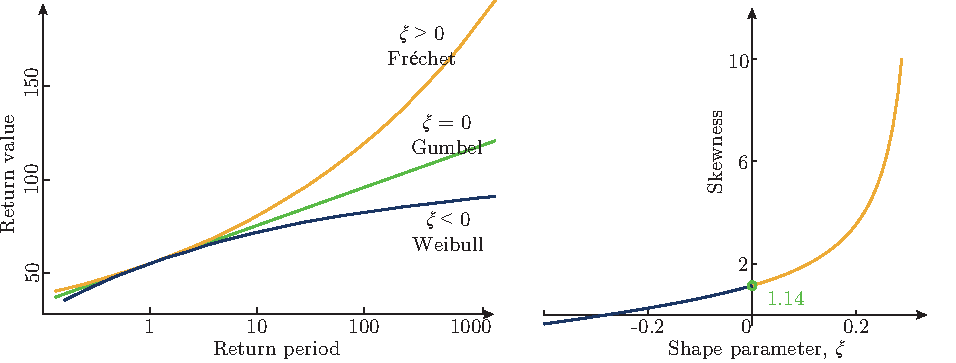
\includegraphics[width=1\textwidth]{GEV_return_value_plot_and_skewness.pdf}
	\caption{Illustration of GEV distribution family in Gumbel space (left), and the related skewness (right).}
	\label{fig:gev_skewness}
\end{figure}

Generalized method of moments (GMM), maximum likelihood (ML), and Bayesian (B) approaches are applied to infer the parameters of the selected distributions. Uncertainty intervals are constructed using delta method, profile likelihood, and bootstrapping in the frequentist paradigm, and highest density and equal tail posterior distribution intervals in the Bayesian one\footnote{These methods and terms are introduced in Chapter~\ref{cha:overview} and in Annex~\ref{sec:stat_tools}.}. An important advantage of the Bayesian approach is that it treats unknown parameters as random variables, hence the incorporation of parameter estimation uncertainty into the model is straightforward. This is done by using the posterior predictive distribution (Eq.\ref{eq:postpred}).

%.......................................................................................
\subsection{Return value--return period plots}

Maximum likelihood method is used to infer the distribution parameters and the results are plotted in Gumbel space (Annex~\ref{sec:prob_plots}). Figure~\ref{fig:loc1_2x2} compares the distribution functions fitted to the observations for Location 1. The edges of the colored ranges are the 90\% confidence intervals obtained by delta method\footnote{The coloring is ``ink-preserving'': the same ``amount of ink'' is used for every vertical section, hence creating a linear transition from the narrowest (dark blue) to the widest interval (white). In a particular 2$\times$2 figure, equal ranges have the same color on each subplot, thus the models are directly comparable based on coloring as well.}. From the plots it is clear that the model type substantially influences the extent of the uncertainty interval. The GEV plot shows that the observations likely belong to the Weibull family and have an upper bound. The other three distributions cannot capture such feature, since they have no upper bound by definition. The difference among the models becomes significant with increasing return period. Similar return value--return period plots are presented in Figure~\ref{fig:loc2_2x2} and \ref{fig:loc3_2x2} for Locations 2 and 3, respectively.

\begin{figure}[htbp!]
	\centering    
	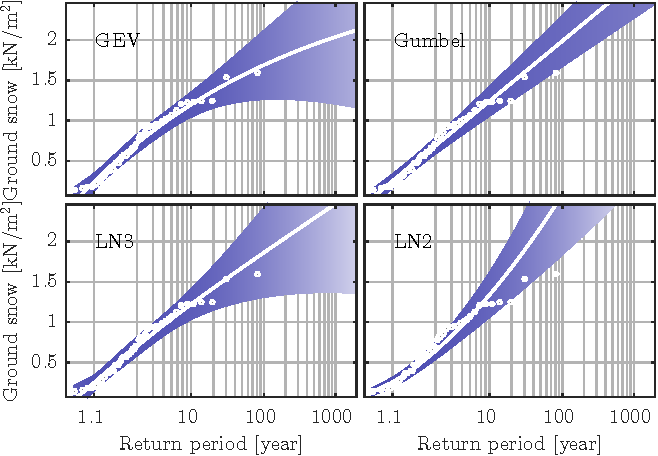
\includegraphics[]{filled_RP_RV_2x2_ID300_CI09.pdf}
	\caption{Location 1 (Weibull-like), ML fitted distributions with 90\% confidence bands (delta method) in Gumbel space.}
	\label{fig:loc1_2x2}
\end{figure}

\begin{figure}[htbp!]
	\centering    
	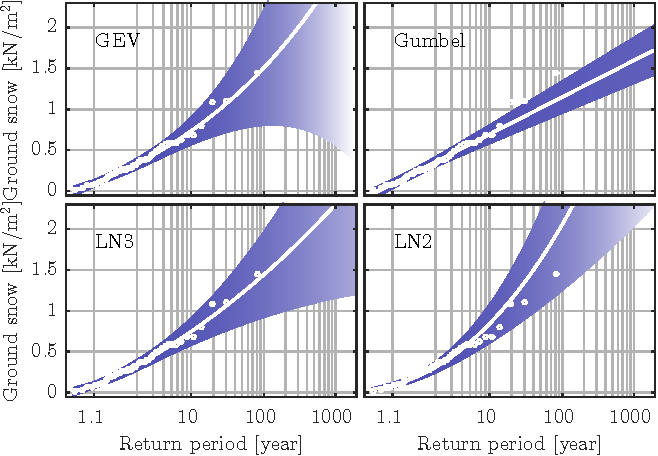
\includegraphics[]{filled_RP_RV_2x2_ID2735_CI09.pdf}
	\caption{Location 2 (Fréchet-like), ML fitted distributions with 90\% confidence bands (delta method) in Gumbel space.}
	\label{fig:loc2_2x2}
\end{figure}

\begin{figure}[htbp!]
	\centering    
	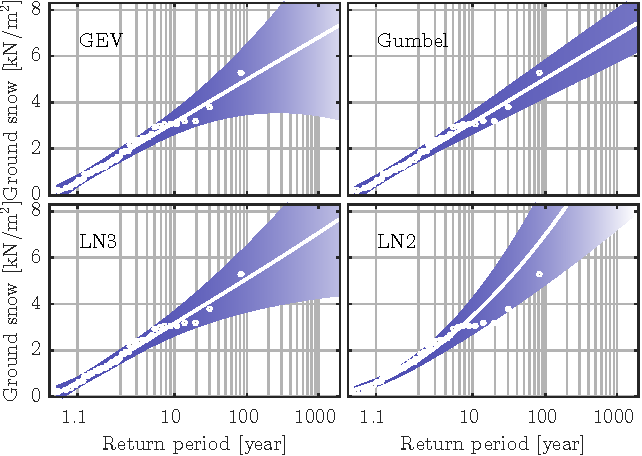
\includegraphics[]{filled_RP_RV_2x2_ID4553_CI09.pdf}
	\caption{Location 3 (Gumbel-like), ML fitted distributions with 90\% confidence bands (delta method) in Gumbel space.}
	\label{fig:loc3_2x2}
\end{figure}

All return value--return period plots -- with the exception of the Gumbel distribution -- show that the confidence interval is rapidly widening as the number of observations reduces and with extrapolation to unobserved region. This is especially salient for the Fréchet-like location (Figure~\ref{fig:loc2_2x2}). Figure~\ref{fig:loc3_2x2} indicates that even if the point estimates are similar, such as for GEV, Gumbel, and LN3, the confidence intervals can be substantially different in the extrapolated region. This information is completely lost if point estimates are considered only. Irrespectively of the location, the Gumbel distribution has significantly narrower confidence interval than the other models. This could be explained by its two parameters, which span smaller space.

By visual inspection the LN3 and GEV distributions seem to provide the best fit; however, in most cases their efficiency can hardly be proven by statistical and information theoretical methods, e.g. using Bayes weights (Eq.\ref{eq:bayes_weight}) or AICc (Eq.\ref{eq:AICc}). On the other hand, the narrow confidence interval of the Gumbel model is unjustified and can be critical in the case of Fréchet-like observations. For Weibull and Gumbel-like samples the LN2 model seems to considerably overestimate the fractiles when compared with the other models.

%....................................................................................
\subsection{Comparing representative fractiles}
To further illustrate the extent and effect of statistical uncertainties, four representative fractiles are inferred using the same four distributions and various methods presented in Chapter~\ref{cha:overview}. Return periods of 50, 100, 300 and 1000 years are selected. When these are interpreted as design point coordinates for the target reliability index of 3.8, then they correspond to sensitivity factors of 0.54, 0.61, 0.71 and 0.81, respectively. Thus, they are approximately representing structures with increasing susceptibility to snow loads; the former two may describe reinforced concrete and the latter two steel structures.

Point estimates with 90\% level uncertainty intervals for Location 1 and 2 are presented in Figures~\ref{fig:loc1_full_summary} and \ref{fig:loc2_full_summary}. The bootstrapping point estimate represents the mean as the mode cannot be estimated directly from the sample. Based on 10 bootstrappings the standard error is less than 1\% for LN2, LN3, and Gumbel distributions. It is about 7\% for large return periods of GEV distribution, which implies that GEV fractiles are more sensitive to sampling variability.

\begin{figure}[htbp!]
	\centering    
	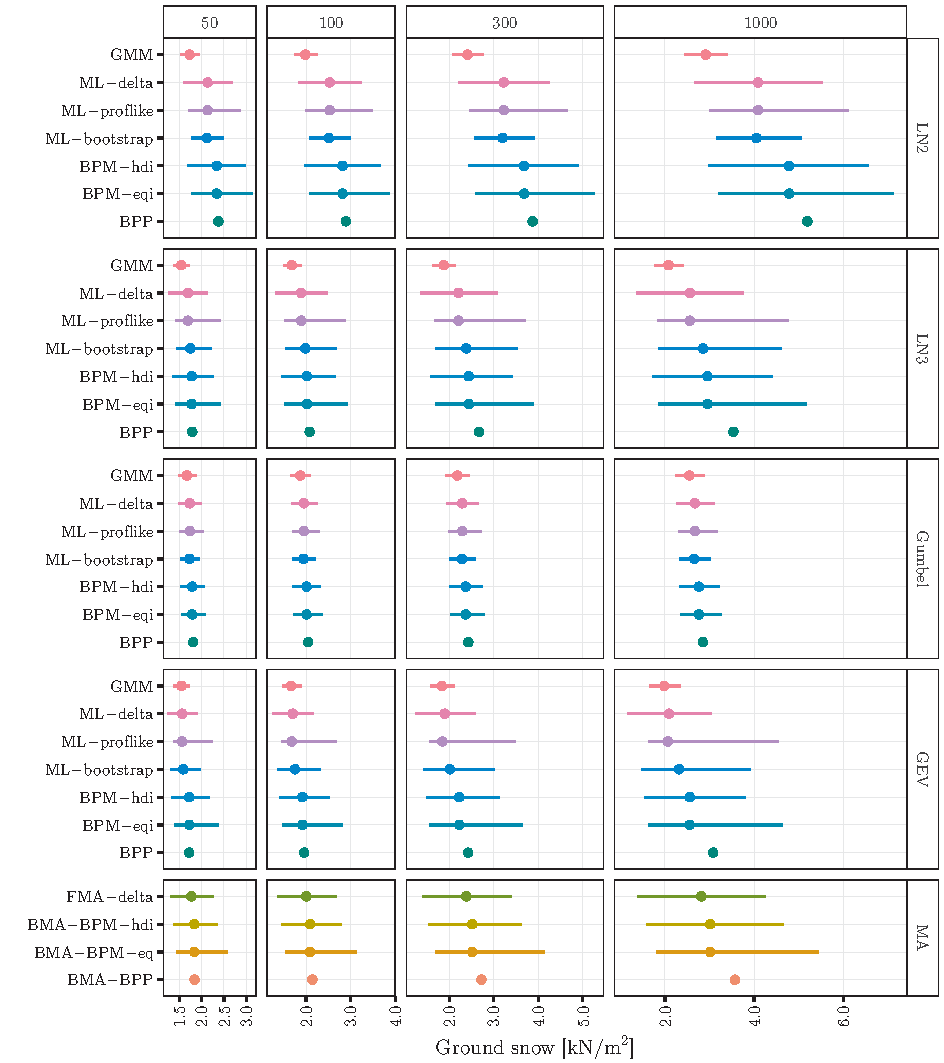
\includegraphics[]{ID300_full_summary_large.pdf}
	\caption{Location 1 (Weibull-like), summary of point estimates and 90\% level uncertainty intervals for the considered models, methods and return periods (notations are explained in Table~\ref{tab:stat_methods_notations}).}
	\label{fig:loc1_full_summary}
\end{figure}


\begin{figure}[htbp!]
	\centering    
	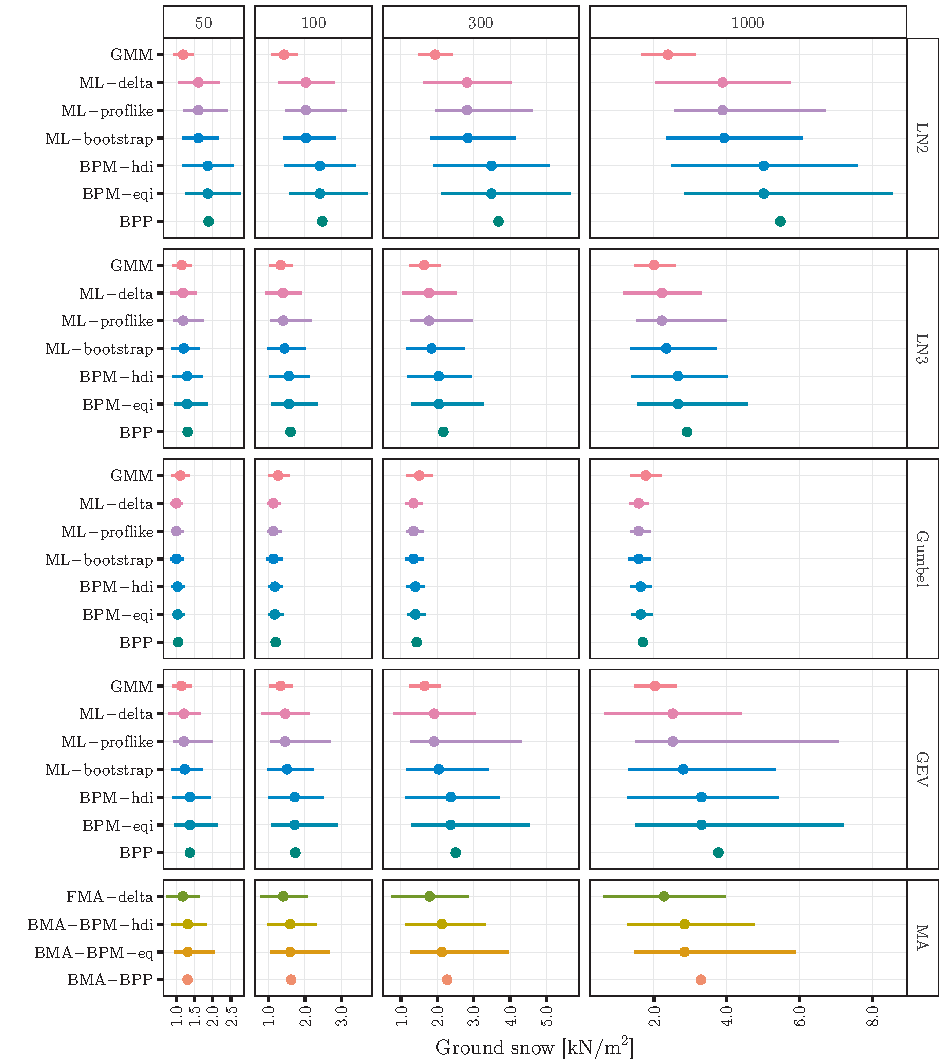
\includegraphics[]{ID2735_full_summary_large.pdf}
	\caption{Location 2 (Fréchet-like), summary of point estimates and 90\% level uncertainty intervals for the considered models, methods and return periods (notations are explained in Table~\ref{tab:stat_methods_notations}).}
	\label{fig:loc2_full_summary}
\end{figure}

For Location 1 the models show considerable difference even for the 50-year return period, for which the uncertainty intervals are relatively narrow. Compared with the Gumbel ML point estimate, the largest difference is observed for the Bayesian posterior predictive estimate of LN2 that is 1.4 times larger. The same ratios for 100, 300 and 1000-year return values are 1.5, 1.7 and 1.9, respectively. The uncertainty and the difference among point estimates for all the distributions become more significant with an increasing return period. The ML and Bayesian methods yield similar point estimates and comparable uncertainty intervals, the largest difference is observed for LN2. The GMM method gives smaller point estimates and narrower intervals than the other methods for Location 1, e.g. for LN3 it is 0.7-0.9 times smaller than the Bayesian posterior mean.

The results of comparative analyses for Location 2 are summarized in Figure~\ref{fig:loc2_full_summary}. This location shows similar trends as of Location 1, but here the difference between Gumbel and the other models increases, particularly in respect of uncertainty intervals.The 1000-year return values based on the LN2, LN3, and GEV models -- using the ML point estimates -- are 2.4, 1.4, 1.6 times larger than that of the Gumbel distribution. %The 1000-year fractile can be considered as the design point coordinate for lightweight steel structures \citep{Holicky2008}.

Besides the uncertainty intervals, the effect of parameter estimation uncertainty is quantified by the ratio of the corresponding posterior predictive and posterior mean fractiles (Table~\ref{tab:loc1_fract_ratio}). The numbers indicate that particularly for GEV and LN3 distributions the effect of this uncertainty becomes significant with increasing return periods. For these the neglect of parameter estimation uncertainty leads to 20\% underestimation of the return value.

\begin{table}[htbp!]
\caption{Location 1 (Weibull-like), ratio of the posterior predictive and posterior mean fractiles.}
\centering
\label{tab:loc1_fract_ratio}
\small
    \begin{tabular}{lllll}
    \toprule
    Return period [year]  & 50 & 100 & 300 & 1000 \\
    \midrule
    \rowcolor{lightgrey} LN2 & 1.02 & 1.03 & 1.05 &	1.09  \\
    LN3	& 1.01 & 1.03 &	1.10 & 1.20  \\
    \rowcolor{lightgrey} Gumbel & 1.01 & 1.02 &	1.02 & 1.03  \\
    GEV & 1.00 & 1.02 &	1.09 &	1.20  \\
   	\rowcolor{lightgrey} BMA & 1.00 & 1.02 &	1.08 & 1.18 \\
    \bottomrule
    \end{tabular}
\end{table}

Return period estimates are compared for models with and without parameter estimation uncertainty in Table~\ref{tab:loc1_reper}. For LN3 and GEV posterior predictive distributions, the return periods are half of those of the posterior mean distributions. The sampling variability has considerable effect on these values, hence they should be treated as indicative.

\begin{table}[htbp!]
\caption{Location 1 (Weibull-like), return periods, derived from posterior predictive distributions corresponding to 1000-year fractiles based on matching posterior mean distributions.}
\centering
\label{tab:loc1_reper}
\small
    \begin{tabular}{lllll}
    \toprule
    Distribution  & LN2 & LN3 & Gumbel & GEV \\
    \midrule
    \rowcolor{lightgrey} Return period & 704 & 436 & 779 &	413  \\
    \bottomrule
    \end{tabular}
\end{table}

The results (Table~\ref{tab:loc1_fract_ratio} and Figure~\ref{fig:loc1_full_summary}-\ref{fig:loc2_full_summary}) show that the distribution type has larger effect on the representative fractiles than the parameter estimation uncertainty. For example for Location 2 the ratios of the 1000-year fractile of the posterior predictive and posterior mean models are 1.09, 1.09, 1.03, 1.14 and 1.16 for LN2, LN3, Gumbel, GEV and MA models respectively. These illustrate the effect of parameter estimation uncertainty.

The model selection uncertainty can be assessed by comparing the posterior mean fractiles for different models. Normalizing the 1000-year fractile of posterior mean models with that of the Gumbel the ratios are 3.05, 1.62, 1.00, 2.01 and 1.73 for LN2, LN3, Gumbel, GEV and MA (model averaged) models respectively. For other locations the trend is similar but less pronounced.

%.......................................................................................
\subsection{Model averaging}
Figures~\ref{fig:loc1_full_summary} and \ref{fig:loc2_full_summary} show that the frequentist (FMA) and Bayesian (BMA) model averaged point and interval estimates yield comparable results, although the frequentist fractiles and intervals tend to be smaller. A more detailed exposition of model averaging of the Bayesian posterior marginals of the fractiles is illustrated in Figure~\ref{fig:loc1_posterior_bma_2x2}. For larger return periods the difference among the models is increasing, thus the model averaged distribution might become multimodal. For Location 1, the Akaike weights are 0.19, 0.20, 0.43 and 0.18 for LN2, LN3, Gumbel, and GEV distributions, respectively. The Bayesian weights given in the same order are 0.13, 0.29, 0.30 and 0.28.

Model averaging certainly provides a better fit than any of the individual models, but since it typically requires considerable additional computational efforts, it is recommended mainly for critical structures and extreme hazards such as nuclear facilities and discharges, rather than common applications.

\begin{figure}[htbp!]
	\centering    
	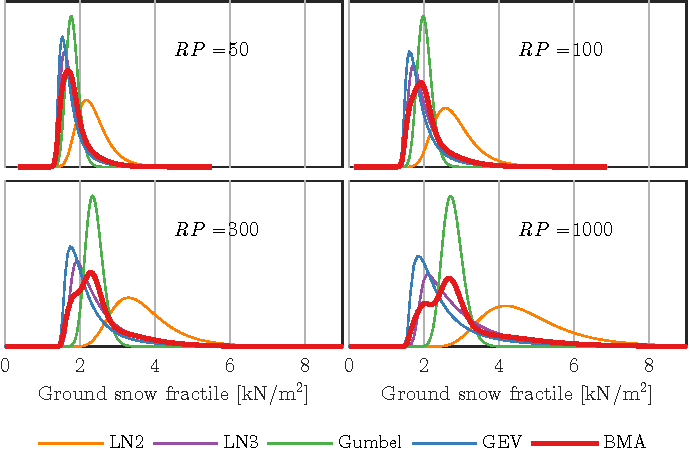
\includegraphics[]{posterior_BMA_2x2_ID300.pdf}
	\caption{Location 1 (Weibull-like), posterior distributions of selected fractiles per different distribution types and Bayesian model averaging.}
	\label{fig:loc1_posterior_bma_2x2}
\end{figure}


%****************************************************************************************
%***************************************************************************************
\section{Effect on structural reliability}
From a practical viewpoint the reliability index is often a more interesting parameter than representative fractiles. Thus the aim of this section is to investigate the effect of statistical uncertainties on structural reliability and to provide practical recommendations regarding their treatment. For this purpose, the reliability level of a generic structural member subjected to snow load is investigated. The effect of parameter estimation and model selection uncertainty in ground snow maxima is considered using frequentist and Bayesian techniques. In contrast with the typically used fixed model and ``best'' point estimates, model averaging and uncertainty intervals are used respectively.

%****************************************************************************************
\subsection{Conceptual framework}
To study the effect of statistical uncertainties, two sets of mechanical-probabilistic models with different representation of the ground snow load are compared. These two model sets are referred hereinafter as \textit{analyzed} and \textit{reference models}, and they differ solely in the ground snow distribution. For example, to illustrate the effect of parameter estimation uncertainty, the \textit{reference model} contains the posterior mean distribution while the \textit{analyzed model} uses the posterior predictive distribution of ground snow. The \textit{reference model} is used to find a mean value of the resistance to reach the target reliability level, which is selected as 3.8 for a considered 50-year reference period. The \textit{analyzed model} has the same mean resistance and thus results based on this model show the effect of different ground snow representation. Throughout this section, different \textit{analyzed-reference model} pairs are considered to illustrate various effects.

The ground snow data of Budapest are used for the analyses (Location 4 in Table~\ref{tab:loc_parmest}). This location  represents lowland areas in the Carpathian Region. Annual maxima from 49 winter seasons are extracted to infer the distributions.

%****************************************************************************************
\subsection{Mechanical and probabilistic model} 

The mechanical model and loads of the analyzed structural member are presented in Figure~\ref{fig:beam_illustration}. The flexural failure of a mid-span cross-section is selected as a representative ultimate limit state:
\begin{equation}
%	\label{eq:BMA}
	g(\mathbf{X}) = {K_{\mathrm{R}}} \cdot R - {K_{\mathrm{E}}} \cdot \left( {\mu  \cdot {s_{{\mathrm{g,50}}}} + {g_{\mathrm{p}}}} \right) \cdot a \cdot \frac{{{L^2}}}{8}.
\end{equation}

\begin{figure}[htbp!]
	\centering    
	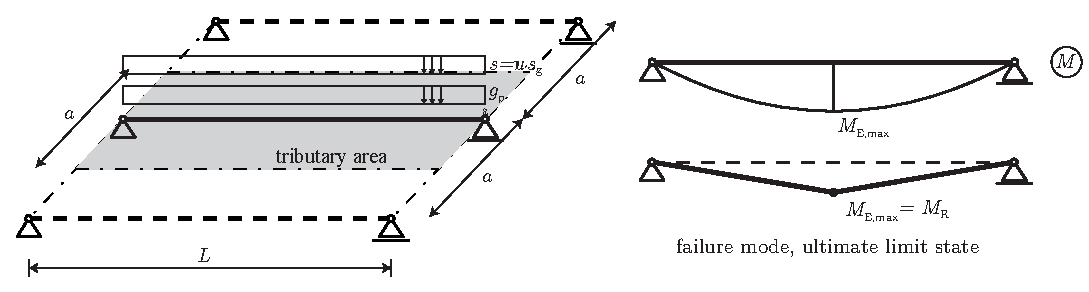
\includegraphics[width = 1\textwidth]{beam_illustration.pdf}
	\caption{Illustration of the analyzed structural member and its failure mode.}
	\label{fig:beam_illustration}
\end{figure}

The variables with their probabilistic model are given in Table~\ref{tab:prob_model_IABSE}. For the annual ground snow load ($s_\mathrm{g,1}$) the sample mean and coefficient of variation ($CV$) are provided since these are also dependent on the fitted distribution type and technique applied to infer parameters of a distribution. The skewness of the analyzed sample is 1.6, indicating Fréchet-type distribution family (Figure~\ref{fig:gev_skewness}). The commonly used Gumbel, Generalized extreme value, two-parameter Lognormal, and three-parameter Lognormal distributions are applied to represent the annual ground snow maxima. The connection between the 1-year and 50-year maxima distributions is established by assuming that the annual maxima are mutually independent.

\begin{table}[htbp!]
\caption{Probabilistic models of simple beam example.}
\centering
\label{tab:prob_model_IABSE}
\small
	\begin{threeparttable}
    \begin{tabular}{l l l l m{3cm}}
    \toprule
    Variable name  & Distribution & Mean & CV & Reference \\
    \midrule
    \rowcolor{lightgrey} Resistance model uncertainty, $K_\mathrm{R}$ [-]  & LN2 & 1.00 & 0.10 & \cite{JCSS_resi} \\
    Resistance, $R$ [kNm] & LN2 & \tnote{*} & 0.15 & \cite{JCSS_resi} \\
    \rowcolor{lightgrey} Load model uncertainty, $K_\mathrm{E}$ [-] & LN2 & 1.00 & 0.10 & \cite{JCSS_load} \\
    Shape factor, $\mu$ [-] & LN2 & 0.80 & 0.17 & \cite{Ellingwood1985} \\
    \rowcolor{lightgrey} Ground snow load, $s_\mathrm{g,1}$ [kN/m$^2$] & \tnote{\textdagger} & 0.4\tnote{\ddag} & 0.7\tnote{\ddag} & \cite{Szalai2013} \\
    Permanent load, $g_\mathrm{p}$ [kN/m$^2$] & N & \tnote{\S} & 0.10 & \cite{JCSS_load} \\
    \rowcolor{lightgrey} Beam span, $L$ [m] & -- & 10 & -- & -- \\
     Bay distance, $a$ [m] & -- & 3 & -- & -- \\
    \bottomrule
    \end{tabular}
    \begin{tablenotes}
    	\item[*] Based on FORM analysis to reach $\beta_\mathrm{target} = 3.8$ with a fixed coefficient of variation.
	    \item[\textdagger] Gumbel, GEV, LN2, LN3, see Appendix~\ref{sec:distr_fun}.
	    \item[\ddag] Using unbiased moment estimates of the sample.
	    \item[\S] Varied to get different load ratios $(\chi)$.
	    \item -- Not applicable/not available.
   	\end{tablenotes}
   	\end{threeparttable}
\end{table}

Different load ratios are achieved by varying the mean value of the permanent load while keeping its coefficient of variation fixed. The load ratio is defined as:
\begin{equation}
	\label{eq:load_ratio}
	\chi  = \frac{{{\mu _{\mathrm{m}}} \cdot {s_{{\mathrm{g,k}}}}}}{{{\mu _{\mathrm{m}}} \cdot {s_{{\mathrm{g,k}}}} + {g_{\mathrm{m}}}}}
\end{equation}
where the m and k subscripts refer to mean and characteristic values respectively.

%****************************************************************************************
\subsection{Statistical analysis}
Frequentist and Bayesian statistical techniques are applied to fit models to the snow maxima and to quantify statistical uncertainties. For the current analysis their most important difference is that the Bayesian approach treats parameters as random variables, thus makes it possible to integrate their estimation uncertainties into the failure probability.

Maximum likelihood and posterior mean are used as point estimates per frequentist and Bayesian approaches respectively. Accordingly, the distributions specified by these point estimates are referred to as maximum likelihood and posterior mean distributions (Table~\ref{tab:stat_methods_notations}).

For the Bayesian calculations vague priors are applied for both to the parameters and to the models as well, and numerical integration is used to calculate the posterior and posterior predictive distributions. Practically infinite ranges are selected for the integrations and uniform priors are adopted on these intervals.

%.......................................................................................
\subsubsection{Results of distribution fitting}
The statistical uncertainties of ground snow models are illustrated on return value-return period plots with confidence bands (Figure~\ref{fig:2546_rp_rv_2x2}). The solid white lines and blue regions show the ML point estimates and 90\% confidence bands respectively; the latter illustrates the parameter estimation uncertainty. The dashed white line and green region correspond to the FMA point estimate and 90\% confidence bands respectively. The extent of model selection uncertainty can be judged by comparing the blue regions to the green ones. For example, for the Gumbel distribution the blue region is considerably wider than the green, this implies that the Gumbel confidence interval is too narrow. This is also supported by the evidence that maxima of the sample are outside of the 90\% confidence band (Figure~\ref{fig:2546_rp_rv_2x2}). This can be observed also for other locations from the CarpatClim database with skewness exceeding 1.2.

\begin{figure}[htbp!]
	\centering    
	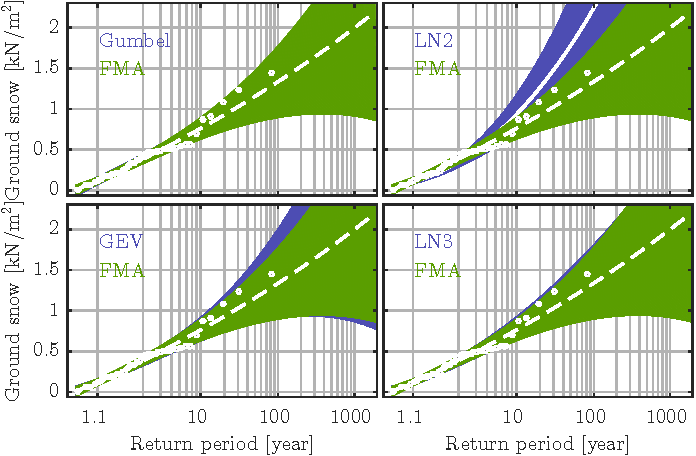
\includegraphics[]{filled_RP_RV_2x2_FMA_ID2546_CI09.pdf}
	\caption{Annual maxima return value--return period plots with 90\% confidence bands for the selected (blue + solid white) and FMA (green + dashed white) distributions in Gumbel space.}
	\label{fig:2546_rp_rv_2x2}
\end{figure}

The Bayesian analysis yields to similar results as the frequentist, although the averaging weights are slightly favoring the three-parameter models over the two-parameter ones (Table~\ref{tab:ma_weights}). Both methods indicate that there is a strong evidence against the LN2 model for this location.

\begin{table}[htbp!]
\caption{Summary of model averaging weights.}
\centering
\label{tab:ma_weights}
\small
    \begin{tabular}{lll}
    \toprule
    Model  & Akaike weight, $w$ & Bayesian weight, $b$ \\
    \midrule
    \rowcolor{lightgrey} GEV  & 0.29 & 0.37 \\
    Gumbel  & 0.43 & 0.25 \\
    \rowcolor{lightgrey} LN3  & 0.28 & 0.38 \\
    LN2  & 0.004 & 0.002 \\
    \bottomrule
    \end{tabular}
\end{table}

Table~\ref{tab:char_snow_bp} shows the characteristic values (0.98 fractile) for the considered models and statistical approaches. With the exception of LN2, which is not supported by the data, the models yield to comparable values. Due to parameter estimation uncertainty the largest increase is observed for LN3, it is about 8\%. The Gumbel model underestimates the model averaged characteristic value by about 10\%. The results for this location are in good agreement with the 1.25 kN/m$^2$ characteristic value specified in the Hungarian National Annex of EN 1991-1-3.

\begin{table}[htbp!]
\caption{Summary of ground snow load characteristic values for Budapest [kN/m$^2$].}
\centering
\label{tab:char_snow_bp}
\small
	\begin{threeparttable}
    \begin{tabular}{l p{3cm} p{3cm} p{3cm}}
    \toprule
    Distribution  & Maximum likelihood (ML) & Bayesian posterior mean (BPM) & Bayesian posterior predictive (BPM) \\
    \midrule
    \rowcolor{lightgrey} GEV  & 1.23 & 1.34 & 1.38  \\
    Gumbel  & 1.07 & 1.11 & 1.12  \\
    \rowcolor{lightgrey} LN3  & 1.20 & 1.18 & 1.28  \\
    LN2  & 1.78 & 1.90 & 1.98  \\
    \rowcolor{lightgrey} FMA & 1.16 & -- & --  \\
   	BMA  & -- & 1.21 & 1.27 \\
    \bottomrule
    \end{tabular}
    \begin{tablenotes}
    	\item -- Not applicable.
    \end{tablenotes}
    \end{threeparttable}
\end{table}

%****************************************************************************************
\subsection{Reliability analysis}

Reliability of the selected structural member is analyzed using the first order reliability method (FORM) considering the various probabilistic representation of the ground snow maxima. Initially a commonly applied Gumbel distribution is investigated. The \textit{reference model} is the Gumbel maximum likelihood distribution, while the analyzed models are the four selected maximum likelihood and the frequentist model averaged distributions. The reliability indices with approximate 90\% confidence bands are presented in Figure~\ref{fig:beta_khi_fma_2x2}. These bands express solely the statistical uncertainties in the ground snow distributions.

This analysis represents the following scenario: Gumbel ML distribution is adopted for snow maxima and a structural member is designed to achieve the target reliability. The failure probability is then calculated assuming that the snow maxima follows other distributions. Figure~\ref{fig:beta_khi_fma_2x2} shows the followings:
\begin{itemize}
	\item The distribution type has substantial effect on the reliability, e.g. for large load ratios the GEV model yields to about 50 times larger failure probability than the Gumbel.
	\item All models yield to smaller reliability index than the \textit{reference} Gumbel.
	\item Compared to the FMA model, the failure probability and uncertainty intervals are largely underestimated by the Gumbel model.
\end{itemize}

\begin{figure}[htbp!]
	\centering    
	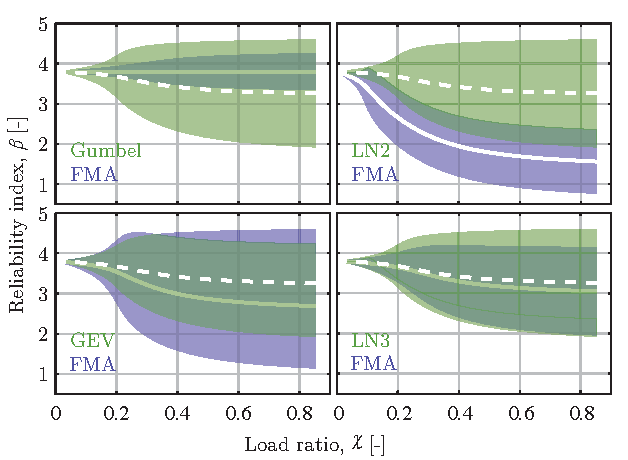
\includegraphics[]{khi_beta_2x2_FMA_ID2546_CI09.pdf}
	\caption{Load ratio–-reliability index plots with 90\% confidence bands for the selected (green + solid white) and FMA (blue + dashed white) ground snow distributions, using Gumbel ML as \textit{reference model}.}
	\label{fig:beta_khi_fma_2x2}
\end{figure}

As the LN2 model is clearly far from the FMA, and not supported by the data (Table~\ref{tab:ma_weights}), it is discarded from the following analyses. The same analysis with BPM models yields to similar results as those of the maximum likelihood based. Since the Bayes weights favor the GEV and LN3 models, the underestimation of Gumbel model is even larger than in the case of FMA.

Figure~\ref{fig:beta_khi_bma_2x2} shows the effect of statistical uncertainties, here the \textit{reference model} is the BPM for each selected model, hence the solid green line is horizontal, indicating the 3.8 value. The \textit{analyzed models} are the BPP and BMA models. The main observations from Figure~\ref{fig:beta_khi_bma_2x2} are as follows:
\begin{itemize}
	\item The effect of parameter estimation uncertainty within the Gumbel model is small; however, the model uncertainty has substantial effect, significantly exceeding an order of magnitude in failure probability.
	\item For GEV and LN3 the consideration of parameter estimation uncertainty gives about 20 and 5 times larger failure probability, respectively.
	\item These effects are rapidly increasing with increasing load ratio and reaching a relatively stable level after ratio of 0.3.
\end{itemize}


\begin{figure}[htbp!]
	\centering    
	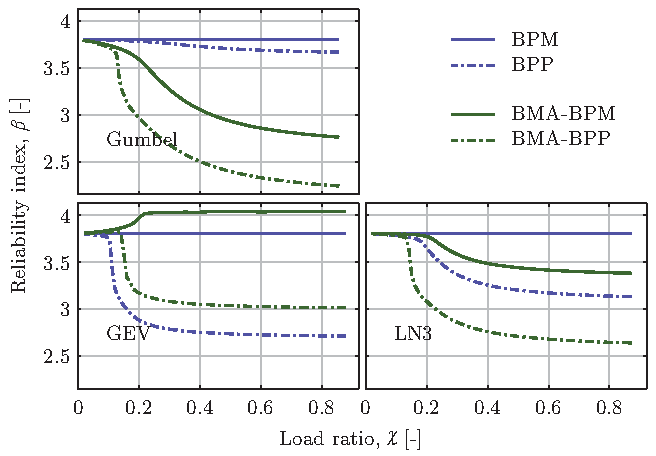
\includegraphics[]{khi_beta_2x2_BPM_BPP_BMA_ID2546_CI09_02.pdf}
	\caption{Load ratio–-reliability index plots for models with (dash-dot) and without parameter estimation uncertainty (solid).}
	\label{fig:beta_khi_bma_2x2}
\end{figure}

Although Table~\ref{tab:char_snow_bp} indicates only minor differences in the characteristic values for the selected probabilistic models, the reliability indices in Figure~\ref{fig:beta_khi_bma_2x2} suggest that the model selection is a key issue for reliability analysis. Consequently, comparison of characteristic values seems to be insufficient to support decision about appropriate probabilistic model.

%\subsection{Extension}

% reference to not detailed works
%75\% confidence interval estimate
%identification of most important component with largest contribution
%\citep{RozsasTVSB2015}


%****************************************************************************************
%****************************************************************************************
\section{Application example: Eiffel-hall of Budapest}

The Eiffel-hall of Budapest is selected to demonstrate the effect of statistical uncertainties on a real life example. The structure is introduced in Annex~\ref{sec:eiffel}, here only the essential details, which are required to interpret the results, are provided. Maximum likelihood method is applied to infer the parameters of annual ground snow maxima of the site. Two-parameter Lognormal, three-parameter Lognormal, Gumbel, and Generalized extreme value distributions are considered for the analysis. The results in terms of reliability indices and normalized failure probabilities are given in Table~\ref{tab:eiffel_statunc}. 50-year reference period is used for all calculations of the structure.

\begin{table}[htbp!]
\caption{Summary of the reliability measures of the selected purlin.}
\centering
\label{tab:eiffel_statunc}
\small
    \begin{tabular}{lllll}
    \toprule
      & Gumbel & GEV & LN2 & LN3 \\
    \midrule
    \rowcolor{lightgrey} $\beta$ & 3.27  & 2.88 & 1.42 & 2.86 \\
    $P_\mathrm{f}/P_\mathrm{f,Gumbel}$ & 1.00  & 3.68 & 145 & 3.96 \\
    \bottomrule
    \end{tabular}
\end{table}

As the site has Fréchet-like distribution with shape parameter greater than zero, all models yield to larger failure probability than that of the Gumbel. The LN3 and GEV failure probabilities are similar and four times larger than that of the Gumbel. The underestimation of Gumbel distribution is more salient for the LN2 distribution that leads to two order of magnitude difference and well represents the significant effect of model selection uncertainty.

%****************************************************************************************
%****************************************************************************************
\section{Discussion}

The main focus of this chapter is the quantification and propagation of statistical uncertainties. From a broader engineering perspective that views reliability analysis as a tool for decision making, the model selection uncertainty problem is recommended to be resolved by agreeing on a conventional distribution type \citep{Melchers2002, Ditlevsen1994}. We support this approach; however, the decision on the selected distribution should be backed by appropriate techniques for model uncertainty analysis. For safety-critical facilities and actions it still might be desirable to analyze this source of uncertainty in detail. The Generalized extreme value distribution is recommended to represent annual maxima of ground snow extremes.This is not a novel recommendation as multiple studies considered GEV or members of GEV family, but for standardization they often settled with other types \citep{Sanpaolesi1998, Ellingwood1984}.

Regarding parameter estimation uncertainty it is argued that it is often advisable to be considered in reliability studies by using the posterior predictive distribution. The main arguments are that reliability analysis is inherently predictive, the failure probability is governed by the very uncertain distribution tails, and after the selection of distribution function it is unambiguous to construct the posterior predictive estimates.
The presented uncertainty interval construction techniques require no or several additional limit state function evaluations as compared to the standard reliability methods such as FORM, and thus are applicable to complex problems as well.

It is argued that in structural reliability every random variable should be represented by its posterior  predictive distribution and for critical cases model averaging should be adopted. This is not a novel in-sight, treatment of statistical uncertainties is well developed in the statistical literature \citep{Wit2012, Aitchison1980} and also advocated in relation to probabilistic engineering analysis \citep{Kiureghian2008, Coles2003fully_prob, Gelder2000}.

The treatment of uncertainties is always related to the  considered  ``model universe'',  i.e.  the  physical and mathematical framework (model) adopted to describe  the  reality.
If point estimates are used the models derived from 5 realizations would convey the same confidence as those based on 1000 data. In contrast, the Bayesian posterior predictive distribution automatically penalizes the small sample size based predictions.
Both presented model averaging (MA) techniques depend on the considered models (the weights in Eq.\ref{eq:bayes_weight}), thus can be interpreted only in respect of the space of selected models.

It should be noted that the results are based on the analysis of few locations with fixed number of observations. For other phenomenon, such as wind extremes, which are typically following Weibull distribution, the effects are anticipated to be smaller. However, smaller number of observations can considerably increase statistical uncertainties. Moreover, it is expected that these uncertainties can be reduced by taking into account more informative priors, which are often available. 

To support future snow maxima related studies the posterior distributions of GEV parameters related to lowlands, and mountains and highlands of the Carpathian Region are calculated and given in Annex~\ref{sec:GEV_posterior}. These can be used as prior information for regions with similar climatic conditions.


%%****************************************************************************************
%%****************************************************************************************
%%\section{Extension to other random variables}
%
%Statistical uncertainties are present for all random variables because they are also inferred from limited observations. The same analysis could be repeated with different distribution types, coefficient of variations or incorporating statistical uncertainties of more random variables.
%\begin{itemize}
%	\item crucial random variables can be identified, e.g. consideration of statistical uncertainties is more important for variable actions than for resistance variables; for wind action, which follows Weibull distribution and has lower coefficient variation than snow loads the effect is less pronounced, for seismic actions it can be even more crucial due to large coefficient of variation \citep{Ellingwood2001}.
%	\item it is valuable if the findings are generalized and extended to other random variables, since the same problems occur.
%\end{itemize}
%
%extensive, at first high quality wind data is available for the Netherlands
%http://www.r-bloggers.com/wind-in-netherlands/


%****************************************************************************************
%****************************************************************************************
\section{Summary and conclusions}

The current practice in civil engineering prevalently overlooks parameter estimation and model selection uncertainties in probabilistic calculations. To assess the effect of this simplification frequentist and Bayesian statistics along with reliability analyses are utilized and the following conclusions are drawn:

\begin{itemize}
	\item The effect of parameter estimation uncertainty within the Gumbel model is small; however, the model uncertainty has substantial effect, considerably exceeding an order of magnitude in failure probability.
	\item The distribution choice may lead to 50 times increase in failure probability (GEV vs. Gumbel).
	\item For the Generalized extreme value and three-parameter Lognormal distributions the consideration of parameter estimation uncertainty can yield to about 20 and 5 times increase in failure probability, respectively.
	\item The use of ``best'' point estimates such as maximum likelihood estimator is not conservative and can have practically significant effect on calculated failure probability.
\end{itemize}

The following practical recommendations and observations are made based on completed analyses:

\noindent For common structures and standardization:
\begin{itemize}
	\item Consensus on the conventional distribution type is needed.  
	\item The commonly applied Gumbel model for annual maxima is often inadequate, this means that it underestimates failure probability and has deceptively narrow uncertainty interval, this model assumption should be revisited.  
	\item Bayesian approach is recommended to handle parameter estimation uncertainties.
\end{itemize}

\noindent For structures that require fully probabilistic risk assessment framework:
\begin{itemize}  
	\item Bayesian statistics is promoted to incorporate both model selection and parameter estimation uncertainties.  
	\item Generalized extreme value distribution is recommended for probabilistic modeling of extremes.
	\item Inclusion of all available data and prior information is recommended; however, guidance on priors is needed.
\end{itemize} 

The consideration of statistical uncertainties can be especially important for predicting extremes under changing climate for which one cannot rely on historical observations.

%The adopted techniques are not restricted to the considered problem and can be utilized for other random variables, phenomena as well, e.g. floods and wind loads.
 
%The applied distribution type has a larger effect on representative fractiles than the parameter estimation uncertainty. Numerical analysis of the annual maxima of ground snow loads reveals that the Gumbel distribution provides unrealistically narrow uncertainty intervals. Use of the generalised extreme value distribution is recommended. The applied parameter estimation technique has considerable effect on the representative fractiles.

%The effect of available observations:
%wind speed study \cite{RozsasREC2016wind}
%stochastic process \ref{cha:copula}
%problems of adaptation and comparison

%The current Eurocode provisions yield to insufficient reliability level if these uncertainties are incorporated, the difference is increasing with increasing snow to dead load ratio.